\section{Durchführung}
\label{sec:Durchführung}
Es wird die in der Abbildung \ref{fig:versuchsaufbau} zu sehende Messapparatur für diesen Versuch verwendet. Als erstes wird eine Nullmessung mit $\SI{1000}{\second}$ durchgeführt und jeweils für die auszusuchenden Proben(Fe, Pb, Al) werden die Dicke $D$ und die Länge $L$ gemessen. 

\begin{figure}[h!]
	\centering
	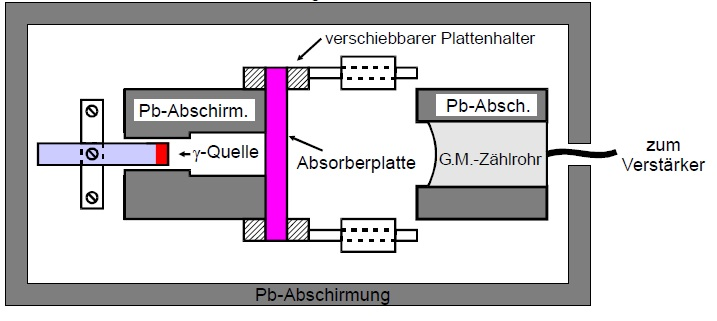
\includegraphics[width=0.7\linewidth]{Versuchsaufbau.jpg}
	\caption{Schematischer Aufbau, \cite[14]{anleitung704}.}
	\label{fig:versuchsaufbau}
\end{figure}

Für die erste Messung wird ein $\gamma$-Strahler($\ce{^137 Cs}$) verwendet, in die Apparatur eingesetzt und für $2$ verschiedene Proben(Pb, Fe) werden $8$ verschiedene Messungen durchgeführt. Bei allen Platten werden die Aktivitäten mindestens $\SI{50}{\second}$ gemessen. Bei den größeren Platten wird eine längere Zeit betrachtet, damit die statistischen Schwankungen so gut wie möglich konstant bleiben. 

Für einen $\beta$-Strahler($\ce{^99 Tc}$), welcher ebenfalls auch in die Apparatur eingesetzt wird, werden $11$ verschiedenen Platten angewendet und zu jedem eine Messung durchgeführt. Bei allen Platten werden die Aktivitäten mindestens $\SI{60}{\second}$ gemessen. 